\section{Dislocation avalanches}Dislocation avalanches can be defined as collective movement of dislocations happening at irregular intervals. 
Dislocations at the nano-scale do not move smoothly,but instead they transition through bursts of activities which are due to dislocation avalanches. $^{\cite{Papanikolaou_2017}}$

Forest dislocations are dislocation in active slip plane which interact with other dislocations having different Burgers vector. These forest dislocations act as pinning point for the movement of the dislocations. When the external force reaches a critical stress, the dislocations lend to overcome the energy barrier by breaking or by jumping over the forest dislocations.$^{\cite{Csikor251}}$.


\begin{wrapfigure}{L}{0.4\textwidth}
\centering
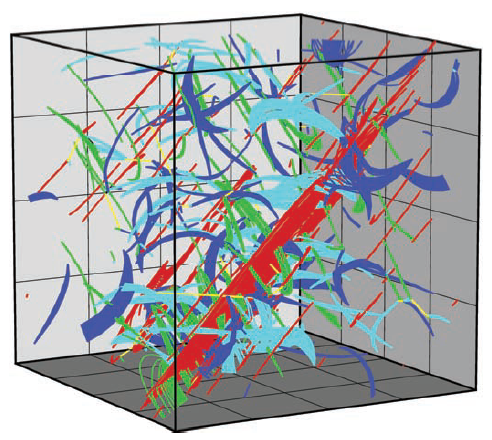
\includegraphics[width=0.35\textwidth]{section_2_1.png}
\caption{\label{fig:Dislocation avalanches}Progress of a large
dislocation avalanche in [010] symmetrical multiple slip for a specimen.$^{\cite{Csikor251}}$}
\end{wrapfigure}


To understand dislocation avalanches. We should understand how dislocation accumulation occurs
\begin{itemize}
  \item Pinning and de-pinning
  \item Jamming or clogging
\end{itemize} 


In pinning and de-pinning, the obstacle are precipitates which impend the dislocation motion. Based on Orowan mechanism which depends on critical radius of the precipitates, the dislocation would cut or loop over the precipitate. The dislocation tend to accumulate at this pinning points. As the external force increases, dislocation jump over the obstacles and get pinned again at other location. The dislocations tend to move collectively in intermittent fashion.
These pinning of dislocation lead to the formation of frank-read mechanism at precipitates which lead to the multiplication of dislocations.

    When the external force reaches a critical stress, the dislocation line would bypass the precipitate by Orowan cutting mechanism. Thus The dislocation line tends to move continuously responds to steady plastic flow.%$^{\cite{425399b347a44656804a82104ffb2a45}}$}
     
Jamming or clogging occurs in caged dynamics. Where the dislocation density is very high. This leads to the dislocation having self-induced constraints to there motion. Jamming or clogging is similar to traffic jams. When the external force is high enough, the dislocation tend to move in a collective manner causing plastic flow.%$^{\cite{425399b347a44656804a82104ffb2a45}}$}


\begin{wrapfigure}{R}{0.35\textwidth}
\centering
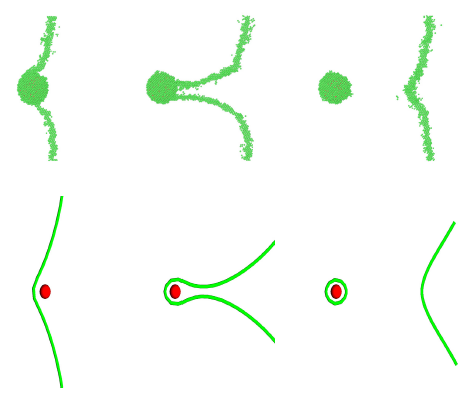
\includegraphics[width=0.3\textwidth]{section_2_2.png}
\caption{\label{fig:Orowan mechanism}Orowan mechanism pinning of dislocation line}%$^{\cite{425399b347a44656804a82104ffb2a45}}$}
\end{wrapfigure}

Grain Boundaries would also acts as barrier to the dislocation motion and impend dislocation until increasing external force causes a collective dislocation glide 
leading to sudden increase in strain-rate in plasticity.This process is repeated until the crack propagation is initiated.$^{\cite{PhysRevB.94.140102}
}$


A quantitative analysis of multi-slip system can be expressed as the number of  dislocation per unit length.The rate at which dislocation density increases is proportional to the number of precipitates. The yield strength can be expressed as the square root of the dislocation density. 
\begin{equation}\label{yield_equation}
\sigma_{y} \propto \sqrt{\rho}
\end{equation}
The equ.(\ref{yield_equation}) shows that as the dislocation density increases, the strength of the material increases.


The atomistic simulation of dislocation avalanches will depend on the pinning point and dislocation density.
The figure (\ref{fig:Dislocation avalanches}) is a simulation of large dislocation avalanche in a symmetrical cube. The lines in red, blue, pink are dislocation avalanche which occurred at different time steps.The yellow lines are the immobile dislocation which act as forest dislocations.

